% Gemini theme
% https://github.com/anishathalye/gemini
%
% We try to keep this Overleaf template in sync with the canonical source on
% GitHub, but it's recommended that you obtain the template directly from
% GitHub to ensure that you are using the latest version.

\documentclass[final]{beamer}

% ====================
% Packages
% ====================

\usepackage[T1]{fontenc}
\usepackage{xcolor}
\usepackage[size=custom,width=200,height=120,scale=2.0]{beamerposter}

\usetheme{acm}
\usecolortheme{acm}
\usepackage{graphicx}
\usepackage{booktabs}
\usepackage{tikz}
\usepackage{pgfplots}
\pgfplotsset{compat=1.14}

% ====================
% Lengths
% ====================

% If you have N columns, choose \sepwidth and \colwidth such that
% (N+1)*\sepwidth + N*\colwidth = \paperwidth
\newlength{\sepwidth}
\newlength{\colwidth}
\setlength{\sepwidth}{0.025\paperwidth}
\setlength{\colwidth}{0.3\paperwidth}

\newcommand{\separatorcolumn}{\begin{column}{\sepwidth}\end{column}}

% ====================
% Title
% ====================

\title{Automating Targeted Password Guessing}

\author{Aravindan Kasiraman \and Bradley Johnson \and Pranav Nair \and Roman Hauksson-Neill \and Sisira Aarukapalli }

% ====================
% Footer (optional)
% ====================

\footercontent{
ACM Research Symposium 2022 \hfill
  \href{https://github.com/ACM-Research/targeted-password-guesses}{https://github.com/ACM-Research/targeted-password-guesses}
   }
% (can be left out to remove footer)


% ====================
% Logo (optional)
% ====================

% use this to include logos on the left and/or right side of the header:
\logoright{\includegraphics[height=7cm]{logo_ACM_Research_light.pdf}}
 \logoleft{\includegraphics[height=7cm]{logo_UTD.pdf}}

% ====================
% Body
% ====================

\begin{document}

\begin{frame}[t]
\begin{columns}[t]
\separatorcolumn
\begin{column}{\colwidth}

  \begin{block}{Introduction}

Imagine trying to hack into your friend's social media account by guessing what password they used to secure it. You do some research to come up with likely guesses – say, you discover they have a dog named "Dixie" and attempt to log in using the password {\tt DixieIsTheBest1}. The problem is that this only works if you have the intuition on how humans choose passwords, and the skills to conduct open-source intelligence gathering.

We refined machine learning models on user data from Wattpad's 2020 security breach to generate targeted password guesses \emph{automatically}. This approach combines the vast knowledge of a 350 million parameter–model with the personal information of 10 thousand users, including usernames, phone numbers, and personal descriptions. Despite the small training set size, our model already produces more accurate results than non-personalized guesses.

  \end{block}

  \begin{block}{Methods}

    In June 2020, Wattpad (an online platform for reading and writing stories) was hacked, and the personal information and passwords of 270 million users were revealed. This data breach is unique in that it connects unstructured text data (user descriptions and statuses) to corresponding passwords. Other data breaches (such as from the dating websites Mate1.com and Ashley Madison) share this property, but we had trouble ethically procuring this data. This data is particularly well-suited for refining a large text transformer like GPT-3, and it's what sets our research apart from a previous study which created a framework for generating targeted guesses using \emph{structured} pieces of user information. The original dataset's passwords were hashed with the bcrypt algorithm, so we used data from the crowdsourced password recovery website Hashmob to match plain text passwords with corresponding user data.
    
    

  \begin{alertblock}{GPT-3 and Language Modeling}

     A language model is a machine learning model that can look at part of a sentence and predict the next word. The most famous language models are smartphone keyboards that suggest the next word based on what you've already typed.

    GPT-3, or Generative Pre-trained Transformer 3, is an artificial intelligence created by OpenAI in February 2019. GPT-3 can translate text, answer questions, summarizes passages, and generate text output on an incredibly sophisticated level. It comes in multiple versions with varying complexity – we used the smallest model "Ada".

  \end{alertblock}

  \end{block}

\end{column}

\separatorcolumn

\begin{column}{\colwidth}
      
    Using GPT-3's fine-tuning API, we showed a pre-existing text transformer model 10 thousand examples for how to correlate a user's personal information with their password.
    
    \includegraphics[width=55cm]{diagram.pdf}
    

  \begin{block}{Results}
    %  \begin{exampleblock}{Password Guesses vs. Actual Passwords}
    %    \centering
    \begin{center}
       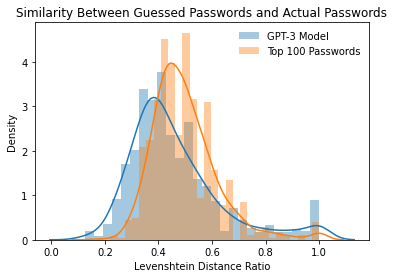
\includegraphics[width=0.49\linewidth]{img/similarity_chart.png}
       \hfill
       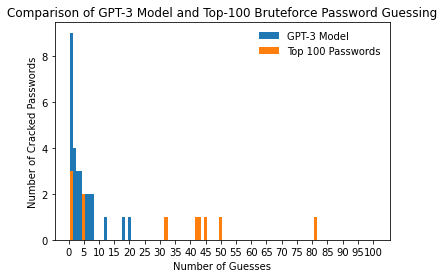
\includegraphics[width=0.49\linewidth]{img/comparison_graph.png}
    \end{center} 
      %  \end{exampleblock}
        
        Using targeted guesses greatly increases the likelihood of not only guessing a target's password, but also guessing passwords that are similar to it. We used the \textbf{Livenshtein distance algorithm} to compute how similar the guessed passwords  are to the target's password. In the figure above, it may seem that the Top 100 Password list performs better on average, but our model has a higher density for Livenshtein ratios of 0.7 and above.
        
        Not only are the GPT-3 model's password guesses more similar to the target's password, but the model is also able to guess more passwords than brute-forcing, and in \textit{significantly less tries}. The second figure shows that our GPT-3 model is often able to guess the target's password \textbf{in less than 10 tries}, whereas the brute-forcing method performs much less consistently.
        
  \end{block}
\end{column}

\separatorcolumn

\begin{column}{\colwidth}

    \begin{block}{Demo}
    
    We created an interactive web demo, so you can see how our model would generate password guesses based on any  information that you input. The backend is built with Flask and directly calls the OpenAI Completion API with our fine-tuned model to generate password guesses based on the inputted personal information.
    
    \begin{columns}
    \begin{column}{0.8\colwidth}
    
     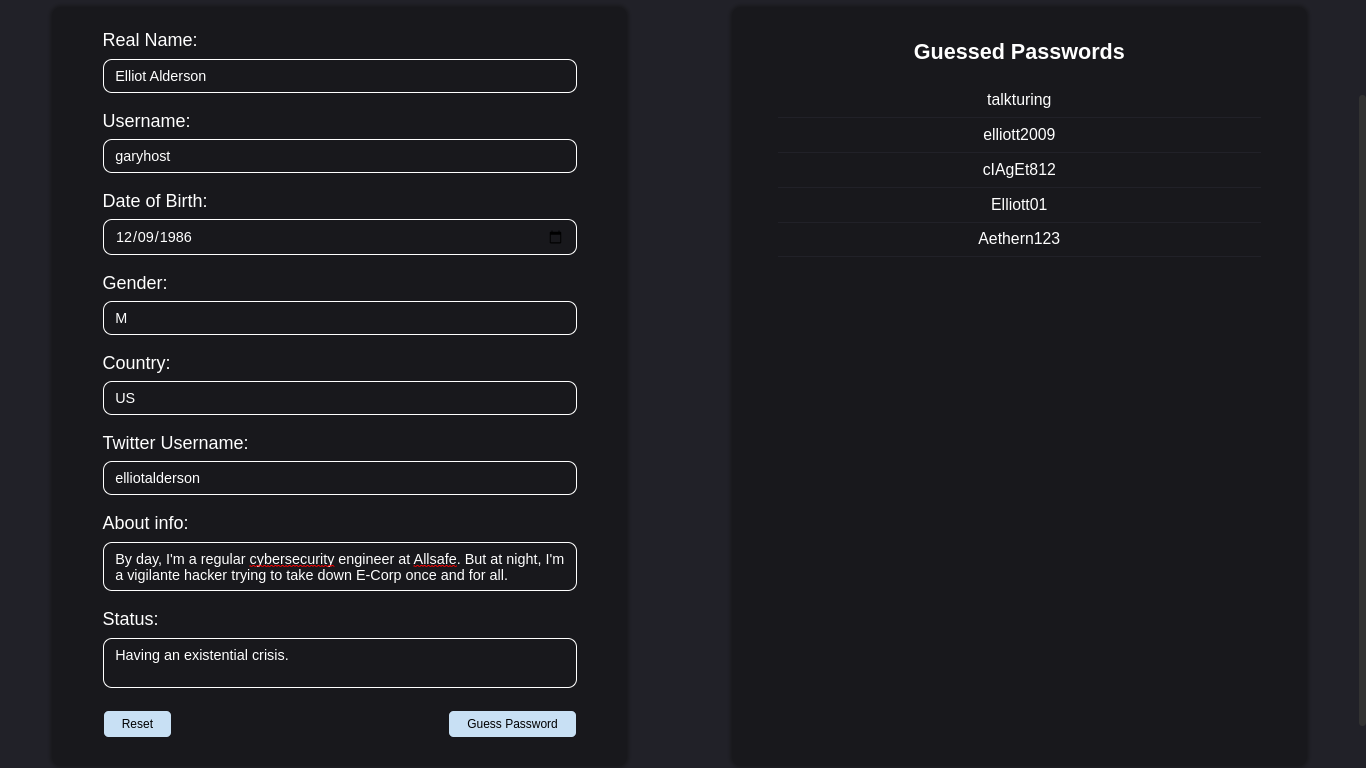
\includegraphics[width=\linewidth]{demo_screenshot.png}
     
    \end{column}
    
    \begin{column}{0.2\colwidth}
    
     
\includegraphics[width=\linewidth]{demo_QR_code.pdf}
     
    \end{column}
    \end{columns}
    
    \end{block}

  \begin{block}{Conclusion}

    Our study reveals both the danger and the utility of accessible advanced machine learning models. With our approach, an attacker could automatically attempt to hack into users' accounts more efficiently than traditional methods, or crack more password hashes from a data leak once brute-force or dictionary attacks reach their effective limit. However, anyone can use this model to see if their passwords are vulnerable, and businesses can run this model on their employees' data to ensure that their company credentials are secure from password guessing attacks. Ultimately, we believe that our use of the GPT-3 model and its effectiveness in generating targeted password guesses can shed light on both existing password practice and future password research.

  \end{block}

  \begin{block}{References}

{\small
    [1] Wang, D., Zhang, Z., Wang, P., Yan, J., Huang, X. (2016). Targeted Online Password Guessing: An Underestimated Threat.
    
    [2] Hitaj, B., Gasti, P., Ateniese, G.,  Perez-Cruz, F. (2019). PassGAN: A Deep Learning Approach for Password Guessing.
    
    [3] Melicher, W., Ur, B., Segreti, S., Komanduri, S., Bauer, L., Christin, N.,  Cranor, L. (2016). Fast, Lean, and Accurate: Modeling Password Guessability Using Neural Networks.
}
  \end{block}

\end{column}

\separatorcolumn
\end{columns}
\end{frame}

\end{document}

